\documentclass{article}
\usepackage[utf8]{inputenc}
\usepackage{graphicx} % allows inclusion of graphics
\usepackage{booktabs}
\usepackage{amsmath}
\usepackage[margin=1.0in]{geometry}
\usepackage{tablefootnote}
\usepackage{listings}
\usepackage{float}

\title{FRIDGe Documentation}
\author{Ryan Stewart}
\date{April 2019}

\begin{document}

\maketitle

\section{Introduction}

The Fast Reactor Input Deck Generator (FRIDGe) is a tool for designing and building input files for MCNP. It grants the user the ability to create elements, materials, assemblies, and full reactor cores. Currently FRIDGe has the ability to create two types of assemblies; blank and fuel assemblies. A blank assembly can be used to build vacant assemblies in a reactor (to simulate experimental areas or holes from control assemblies). A fuel assembly can be used to build a multiple types of driver assemblies or blanket assemblies. FRIDGe currently contains 24 elements which are most commonly used in the development of fast reactors. Along with this, there are 8 base material for us in FRIDGe. There are also examples of both assembly and core files.

\section{Data}

\subsection{Chart of the Nuclides}

To create materials in FRIDGe, the corresponding elements must be present in the directory \verb|fridge/data/CotN|. Each element needs is own YAML file and contains seven variables for inputting data; where each variable and its associate input can be seen in Table \ref{tab:element}

\begin{table}
	\centering
	\caption{Variables for Element YAML file.}
	\begin{tabular}{lcccc}\toprule
		Variable Name   & Variable Type & Unit & Example 
		\\
		\hline
		Name  & string & -- & Silicon
		\\
		ZAID & integer &-- & 14000
		\\
	    Isotopes & list of integers & --& [14028, 14029, 14030]
		\\
		Abundance & list of floats & wt \% & [0.92223, 0.04685, 0.0392]
		\\
		Mass & list of floats &  amu & [27.976926, 28.976494, 29.973777]
		\\
		Density & float & g/cc & 2.33
		\\
		Linear Coefficient of Expansion & float & $K^{-1}$ &0.0
		\\
		\bottomrule
	\end{tabular}
	\label{tab:element}
\end{table}

\verb|Name| is a string containing the name of the element. \verb|ZAID| is an integer denoted by 1000 * Z (proton or atomic number). \verb|Isotopes| is a list of ZAID's for each isotope in the element denoted by 1000 * Z + N, where N is the mass number (protons + neutrons) of the isotope. \verb|Abundance| is a list of the natural abundances for the isotopes (this is in weight percent and can be found in any Chart of the Nuclide). Note: for elements with no natural abundances an entry of zero is allowed. The abundance can be set later in the material card. \verb|Mass| is a list of nuclide masses for each isotope listed and is given in amu's. All abundances and masses were obtained using IAEA's Live Chart of Nuclides \cite{CotN}. \verb|Density| is the density of the natural isotope in g/cc. \verb|Linear Coefficient of Expansion| is the coefficient of thermal expansion and is in units of $K^{-1}$.

\subsection{Material}

Materials can be found in the directory \verb|fridge/data/materials|. Each material in a problem requires its own YAML file and contains five mandatory variables and three optional variables. Where each variable and its associate input can be seen in Table \ref{tab:element}

\begin{table}
	\centering
	\caption{Variables for Material YAML file.}
	\begin{tabular}{lcccc}\toprule
		Variable Name   & Variable Type & Unit & Example 
		\\
		\hline
		Name  & string & -- & UO2
		\\
		Elements & list of str & -- & ['U', 'O]
		\\		
		ZAIDs & list of ints & -- & [92000, 8000]
		\\
	    Weight Fractions & list of floats & wt\% & [0.881467, 0.118533]
		\\
		Enrichment ZAIDs$^*$ & list of ints & -- & [92000, 8000]
		\\
		Enrichment Isotopes$^*$ & list of list of ints & -- & [[92235, 92238], [8016]]
		\\
		Enrichment Vector$^*$ & list of list of floats & wt\% & [[ 0.03, 0.97], [1.0]]
		\\		
		Density & float & g/cc & 2.33
		\\
		Linear Coefficient of Expansion & float & $K^{-1}$ &0.0
		\\
		\bottomrule
	*Optional variables if material has specific isotopics.
	\end{tabular}
	\label{tab:material}
\end{table}

\verb|Name| is a string containing the name of the element. \verb|Elements| is a list of element symbols to be used in the material. Note: This element symbol is how FRIDGe finds the element in \verb|fridge/data/CotN|, so ensure that the elements exists there and the symbol matches.
\verb|ZAIDs| is list of an integers, where each ZAID is denoted by 1000 * Z (proton or atomic number). \verb|Weight Fractions| is a list of floats whose entries are the weight fractions associated with the \verb|ZAIDs| above. Note: This value should sum to 1.0. \verb|Enrichment ZAIDs| is a list of ZAIDs whose isotopic fraction is different from the base element. Note: If the isotopic composition is the same as the element in question, the element does not need to be included and it will be created as normal. \verb|Enrightment Isotopes| is a list of lists of isotopic ZAIDs, where each list corresponds to the the the \verb|Enrichment ZAIDs| from above. \verb|Enrichment Vector| is a list of lists of weight fractions (enrichment) of each isotope from \verb|Enrichment Vector|. Note: Each list should sum 1.0. \verb|Density| is the density of the natural isotope in g/cc. \verb|Linear Coefficient of Expansion| is the coefficient of thermal expansion and is in units of $K^{-1}$

\subsection{Assembly}

There are two types of assemblies that can be built in FRIDGe; blank and fuel assemblies. Both types of assemblies are created using YAML files and can be found in \verb|fridge/data/assembly|. Assembly files for blank and fuel requires a different number of variables; the required variables can be seen in Table \ref{tab:blank} and Table \ref{tab:fuel}.

\begin{table}
	\centering
	\caption{Variables for Blank Assembly YAML file.}
	\begin{tabular}{lcccc}\toprule
		Variable Name   & Variable Type & Unit & Example 
		\\
		\hline
		Assembly Type  & string & -- & Blank
		\\
		Assembly Pitch & float  & cm & 12.0
		\\		
		Duct Thickness & float & cm & 0.3
		\\
	    Duct Inside Flat to Flat & float & cm & 11.1
		\\
		Assembly Height & float & cm & 240
		\\
		Coolant & string & -- LiquidNa
		\\
		Assembly Material & string & -- & HT9
		\\		
		Blank Height & float & cm & 220
		\\
		Blank Smear & Dictionary & {str: wt \%} & {LiquidNa: 0.9, HT9: 0.1}
		\\
		Z Position & float & cm & -60
		\\
		\bottomrule
	\end{tabular}
	\label{tab:blank}
\end{table}

\verb|Assembly Type| is a string used to denote the types of assembly (blank or fuel). \verb|Assembly Pitch| is a float to denote the distance from the center of one assembly to an adjacent assembly. Note: All assemblies in a core should have the same assembly pitch; if they don't errors in geometry may arise. \verb|Duct Thickness| is a float do denote the thickness of the assembly duct. \verb|Duct Inside Flat to Flat| is a float to denote the distance from one side of a hexagon to the other. \verb|Assembly Height| is a float used to denote the total height of the assembly. \verb|Coolant| is a string used to create a material for the coolant. \verb|Assembly Material| is a string used to create a material for the assembly. \verb|Blank Height| is a float used to denote the height of the blank portion of the assembly. Note: If \verb|Blank Height| of the assembly exceeds the \verb|Assembly Height|, the \verb|Assembly Height| will truncate the \verb|Blank Height|, this may lead to geometry errors. \verb|Blank Smnear| is a dictionary of strings and weight percents. This will create a smeared material where each string in the dictionary will create a material, whose weight fraction is the corresponding float. \verb|Z Position| is a float which allows the user to manually adjust where they want the bottom of the blank assembly to be.

\begin{table}
	\centering
	\caption{Variables for Fuel Assembly YAML file.}
	\begin{tabular}{lcccc}\toprule
		Variable Name   & Variable Type & Unit & Example 
		\\
		\hline
		Assembly Type  & string & -- & Blank
		\\
		Assembly Pitch & float  & cm & 12.0
		\\		
		Duct Thickness & float & cm & 0.3
		\\
	    Duct Inside Flat to Flat & float & cm & 11.1
		\\
		Assembly Height & float & cm & 240
		\\
		Coolant$^{*,**}$ & string & -- LiquidNa
		\\
		Assembly Material & string & -- & HT9
		\\
		Pins Per Assembly & int & -- & 271
		\\
		Pin Diameter & float & cm & 0.53
		\\
		Clad Thickness & float & cm & 0.037 
		\\
		Fuel Smear$^\dagger$ & float & \% & 0.75
		\\
		Fuel Diameter$^\dagger$ & float & cm & 0.5
		\\		
		Pitch & float & cm & 0.661
		\\		
		Wire Wrap Diameter & float & cm & 0.126
		\\
		Wire Wrap Axial Pitch & float & cm & 2.0
		\\
		Fuel Height & float & cm & 60
		\\
		Fuel & str & -- & UO2
		\\
		Clad & str & -- & HT9
		\\
		Bond & str & -- & LiquidNa
		\\
		Bond Above Fuel$^*$ & float & cm & 0.6
		\\
		Plenum Height & float & cm & 220
		\\
		Plenum Smear & dictionary & {str: wt \%} & {LiquidNa: 0.5, HT9: 0.25, Void: 0.25}
		\\
		Reflector Height & float & cm & 220
		\\
		Reflector Smear & dictionary & {str: wt \%} & {LiquidNa: 0.5, HT9: 0.25, Void: 0.25}
		\\
		\bottomrule
	\end{tabular}
	\\
	$\dagger$ Either fuel smear or fuel diameter can be used.
	\\
	* Optional
	\\
	** Required if building a single assembly.
	\\	
	\label{tab:fuel}
\end{table}

\verb|Assembly Type| is a string used to denote the types of assembly (blank or fuel). \verb|Assembly Pitch| is a float to denote the distance from the center of one assembly to an adjacent assembly. Note: All assemblies in a core should have the same assembly pitch; if they don't errors in geometry may arise. \verb|Duct Thickness| is a float do denote the thickness of the assembly duct. \verb|Duct Inside Flat to Flat| is a float to denote the distance from one side of a hexagon to the other. \verb|Assembly Height| is a float used to denote the total height of the assembly. \verb|Coolant| is a string used to create a material for the coolant. \verb|Assembly Material| is a string used to create a material for the assembly. \verb|Pins Per Assembly| is an integer of the number of pins for the assembly. Note: This number should fit an exact number of rings required, Table \ref{tab:rings}, shows pins are required for a given number of rings.

\begin{table}
	\centering
	\caption{Hexagonal Rings to Pins/Assemblies.}
	\begin{tabular}{lc}\toprule
		Number of Rings & Number of Pins/Assemblies 
		\\
		\hline
		One  & 1 
		\\
		Two & 7
		\\
		Three & 19 
		\\
		Four & 37
		\\
		Five & 61 
		\\
		Six & 91
		\\
		Seven & 127
		\\
	    Eight & 169
		\\
		Nine & 217 
		\\
		Ten & 271
		\\
		Eleven & 331
		\\		
		\bottomrule
	\end{tabular}
	\label{tab:rings}
\end{table}

\verb|Pin Diameter| is a float which is the diameter of the fuel pin (outside of the cladding). \verb|Clad Thickness| is a float to denote the cladding thickness. \verb|Fuel Smear| is a float to denote the percentage of area inside the cladding that the fuel encompasses, the relation between the fuel diameter and fuel smear can be seen below, where $R_{IC}$ is the inner cladding radius, and $A_fuel$ is the \verb|Fuel Smear|.

\begin{equation}
    R_{fuel} = \sqrt{\%A_{fuel}}R_{IC}
\end{equation}

\verb|Fuel Diameter| is a float to denote the diameter of the fuel slug. \verb|Pitch| is a float to denote the distance from the center of one fuel pin to an adjacent fuel pin. \verb|Wire Wrap Diameter| is a float to denote the diameter of the wire wrap. Note: The diameter of the pin plus the diameter of the wire wrap should not exceed the pitch. FRIDGe will allow this, but it is not physically possible. \verb|Wire Wrap Axial Pitch| is a float which denotes the distance between each wrap. \verb|Fuel Height| is a float to denote the height of the fuel pin. \verb|Fuel| is a string to denote the fuel material. \verb|Clad| is a string to denote the cladding material. \verb|Bond| is a float to denote the fuel bond material. \verb|Bond above Fuel| is a float to denote the height of the bond above the fuel. 
\verb|Plenum Height| is a float used to denote the height of the plenum portion of the assembly.  \verb|Plenum Smear| is a dictionary of strings and weight percents. This will create a smeared material where each string in the dictionary will create a material, whose weight fraction is the corresponding float. \verb|Reflector Height| is a float used to denote the height of the reflector portions of the assembly.  \verb|Reflector Smear| is a dictionary of strings and weight percents. This will create a smeared material where each string in the dictionary will create a material, whose weight fraction is the corresponding float.

\subsection{Core}

A core is built by placing any number of assemblies into any position within the core. It is created using a YAML file, which can be found in \verb|fridge/data/core| and requires four variables in addition to $n$ number of assembly positions. \ref{tab:core} shows the requirements for a core file.

\begin{table}
	\centering
	\caption{Variables for Core YAML file.}
	\begin{tabular}{lcccc}\toprule
		Variable Name   & Variable Type & Unit & Example 
		\\
		\hline
    	Name  & string & -- & TestCore
		\\
		Vessel Thickness & float & cm & 10.0
		\\		
		Vessel Material & string & -- & HT9
		\\
		Coolant Material & string & -- & LiquidNa
		\\
	    Assembly Positions & dictionary & str: str & 01A01: TestAssembly
		\\
		\bottomrule
	\end{tabular}
	\label{tab:core}
\end{table}

\verb|Name| is a string used to denote the name of the core. \verb|Vessel Thickness| is a float do denote the thickness of the vessel both axially and radially. \verb|Vessel Material| is a string used to create a material for the reactor vessel. \verb|Coolant Material| is a string used to create the coolant for the reactor vessel. Note: This will overwrite any coolant material assigned to an assembly. \verb|Assembly Position| is used to describe each assembly in the core, and what assembly goes there. The first entry is a five character string which broken into a triplet. The first two number denote the ring, the letter denotes the hextant, and the last two numbers denote the number of assemblies off the hextant axis. Figure \ref{fig: Core}, shows the nomenclature used to describe each position.

\begin{figure}
    \centering
    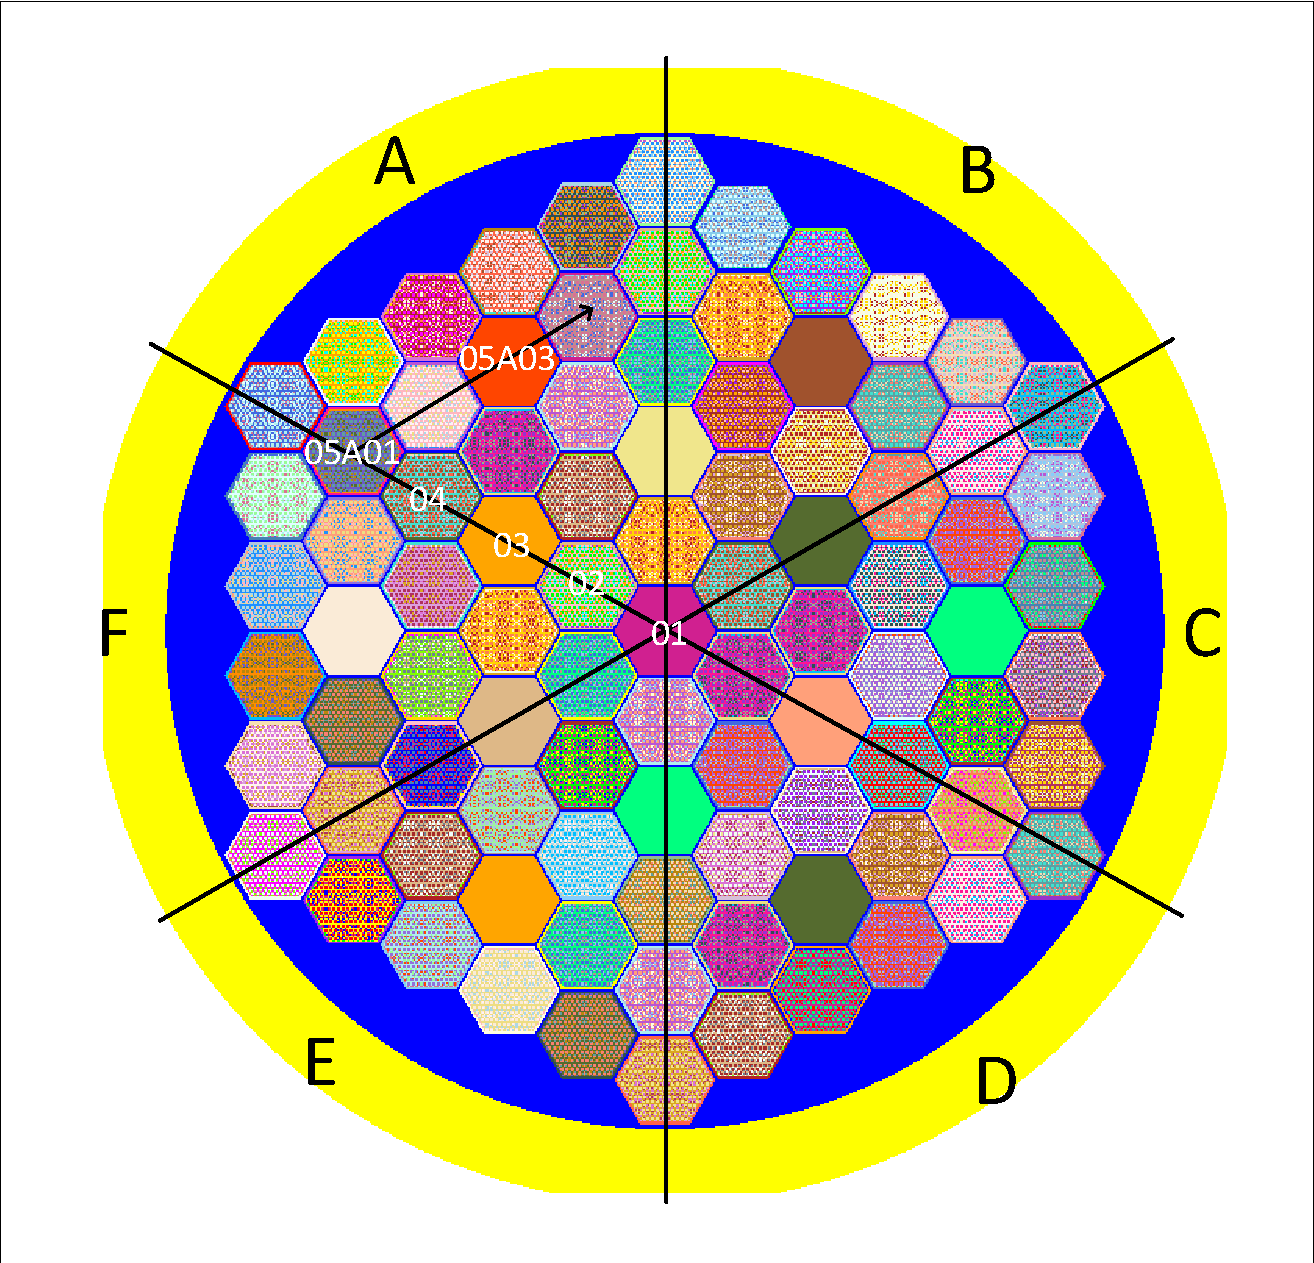
\includegraphics[width=0.65\textwidth]{FullCore.pdf}
    \caption{Description of assembly positions.}
    \label{fig: Core}
\end{figure}

\subsection{FRIDGe Input File}

The FRIDGe input file is used to denote general properites for the MCNP input file, and what core/assembly to make, these files can be found int \verb|fridge/fridge_input_files|. There are currently 16 options that can be included in the FRIDGe input file, Table \ref{tab:input} gives a descriptions of each one and the default value.

\begin{table}
	\centering
	\caption{Variables for FRIDGe Input YAML file.}
	\begin{tabular}{lcccc}\toprule
		Variable Name   & Variable Type & Unit & Example & Default 
		\\
		\hline
    	Name  & string & -- & FRIDGe\_Test & 
		\\
    	Input Type  & string & -- & Core & Single
		\\
    	Output File Name$^*$  & string & -- & File23 & FRIDGe1
		\\				
		Temperature$^*$ & int & K & 1200 & 900
		\\		
		XC Library$^*$ & string & -- & ENDFVII.0 & ENDFVII.1
		\\
		Number of Generations$^*$ & int & -- & 1000 & 230
		\\
		Number of Skipped Generations$^*$ & int & -- & 50 & 30
		\\	
		Number of Particle Per Generations$^*$ & int & -- & 1e8 & 1e6
		\\			
	    Run Kinetics$^*$ & Boolean & -- & True & False
		\\
		Void Percent$^*$ & float & \% & 0.1 & 1.0
		\\	
	    ksens$^{*,**}$ & Boolean & -- & True & False
		\\
	    Temperature Adjusted Density$^{*,**}$ & Boolean & -- & True & False
		\\
	    Temperature Adjusted Volume$^{*,**}$ & Boolean& -- & True & False
		\\
	    Smear Clad$^{*,**}$ & Boolean & -- & True & False
		\\	
	    Smear Bond$^{*,**}$ & Boolean & -- & True & False
		\\
		\bottomrule
	\end{tabular}
	\\
	* Optional
	\\
	** Currently not built into FRIDGe.
	\label{tab:input}
\end{table}

The only variables required for building a FRIDGe input file are the \verb|Name| and \verb|Input Type|, all other variables have default setting. The \verb|Name| is assembly or core file which will be used. The \verb|Input Type| is the the type of file to be create, two options are available; Single and Core. \verb|Output File Name| will denote the name of the MCNP input file, \verb|.i| file, that will be created. \verb|Temperature| is the temperature of the system denoted in Kevlin, currently there are three options; 600, 900, and 1200. \verb|XC Library| is the name of the cross section library that will be used, currently there are three options; ENDFVII.0, ENDFVII.1, JEFF3.1. Note: The combination of \verb|Temperature| and \verb|XC Library| will select the appropriate cross-section set for each material used. \verb|Number of Generations| is the MCNP number of generations that the simulation will run for. \verb|Number of skikpped Generations| is the MCNP number of generations that are skipped before statistics are started. \verb|Number Particles per Generation| is the number of particles that will be run for each generation. \verb|Run Kinetics| will implement the \verb|kopts| portion of code for MCNP, the default setting for \verb|kopts| are currently used. The remaining settings are currently not used in FRIDGe, but are intended for addition. A description of each will be added as each variable is added.

\section{Test Suite}

FRIDGe has an a test suite built that can be run to ensure all of the packages are operating correctly. To run the test suite, open a terminal in the fridge directory and perform the following:

\begin{lstlisting}
python -m pytest
\end{lstlisting}

This should run all of the files in \verb|fridge/test_suite|. There are currently 82 tests which need to be run. This will generate four MCNP input files in \verb|fridge/mcnp_input_files|. Note: There are four MCNP input files with the preface \verb|Prefab_|, these are the MCNP input files that the test suite is checking against. DO NOT alter these files in any way.

\subsection{Fuel Assembly Example}

An few example fuel assemblies can be seen in \verb|fridge/data/assembly|. This example will look at the \verb|EBRII_MKII| assembly. This assembly has the following attributes, which can be seen in Table \ref{tab:ebrii}.

\begin{table}[H]
	\centering
	\caption{Variables for Fuel Assembly YAML file.}
	\begin{tabular}{lc}\toprule
		Variable Name   & EBRII MKII Assembly
		\\
		\hline
		Assembly Type  & Fuel 
		\\
		Assembly Pitch & 5.887 
		\\		
		Duct Thickness & 0.2032 
		\\
	    Duct Inside Flat to Flat & 5.6134 
		\\
		Assembly Height & 164.386 
		\\
		Coolant & LiquidNa 
		\\
		Assembly Material & SS316
		\\
		Pins Per Assembly & 91 
		\\
		Pin Diameter & 0.4420 
		\\
		Clad Thickness & 0.0305
		\\
		Fuel Diameter & 0.3302
		\\		
		Pitch & 0.566
		\\		
		Wire Wrap Diameter & 0.124
		\\
		Wire Wrap Axial Pitch & 15.24 
		\\
		Fuel Height & 34.29 
		\\
		Fuel & U
		\\
		Clad & SS316 
		\\
		Bond & LiquidNa 
		\\
		Bond Above Fuel & 1.31 
		\\
		Plenum Height & 28.3
		\\
		Plenum Smear & {LiquidNa: 0.50, Void: 0.25, SS316: 0.25} 
		\\
		Reflector Height & 61.3537 
		\\
		Reflector Smear & {LiquidNa: 0.116, 0.884} 
		\\
		\bottomrule
	\end{tabular}
	\label{tab:ebrii}
\end{table}

The inputs from \ref{tab:ebrii} create an assembly similar to the MK-II driver assemblies found in EBRII, as referenced in \cite{ebrii}, where Figures \ref{fig: fullAssem} - \ref{fig: fuelRegion} show the MCNP assembly. In Figure \ref{fig: fullAssem} the regions are, from bottom to top; lower reflector, fuel, plenum and upper reflector. In \ref{fig: upperFuel}, we see the impact of including the variable \verb|Bond Above Fuel|, which adds the bond material (blue) above the fuel (purple). Figure \ref{fig: fuelRegion} shows the 91 pins in the assembly; there is fuel (purple), bond (blue), clad (yellow), wire wrap + coolant mixture (green), excess coolant (light blue), and the hex duct (maroon).

\begin{figure}
    \centering
    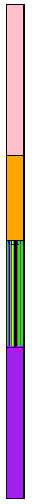
\includegraphics[width=0.05\textwidth]{EBRII_Assembly.PNG}
    \caption{View of entire length of an EBRII assembly.}
    \label{fig: fullAssem}
\end{figure}
\begin{figure}
    \centering
    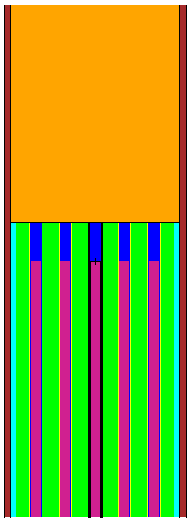
\includegraphics[width=0.25\textwidth]{EBRII_UpperFuel.PNG}
    \caption{Sodium above fuel height.}
    \label{fig: upperFuel}
\end{figure}
\begin{figure}
    \centering
    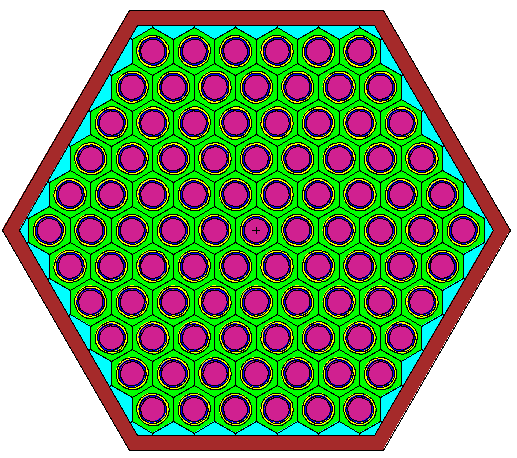
\includegraphics[width=0.55\textwidth]{EBRII_FuelSection.PNG}
    \caption{Fuel region of EBRII assembly.}
    \label{fig: fuelRegion}
\end{figure}

\section{Running FRIDGe}

Running FRIDGe is best done in an interactive python terminal (such as ipython). Once an Ipython terminal is open in the \verb|fridge| directory, import \verb|fridfe_driver| as follows:
\begin{verbatim}
    import fridge.driver.fridge_driver as fd
\end{verbatim}
To run a FRIDGe input file, run the \verb|main| program with the input file name as a string input, as seen below. Note: You do not include the file type.
\begin{verbatim}
     fd.main('<input file name>')
\end{verbatim}
For example the EBRII assembly that was created in the previous section can be run as follows:
\begin{verbatim}
     fd.main('EBRII_Driver')
\end{verbatim}
Users can now continue to make material, assembly, core, and FRIDGe input files. These corresponding MCNP input files will be listed in \verb|/fridge/mcnp_input_files/| with the given output file name specified int eh FRIDGe input file.

\begin{thebibliography}{}
\bibitem{CotN}
    "Livechart - Table of Nuclides - Nuclear structure and decay data", Www-nds.iaea.org, 2019. Available: https://www-nds.iaea.org/relnsd/vcharthtml/VChartHTML.html. [Accessed: 01- May- 2019].
\bibitem{ebrii}
    E. Lum, C. Pope, R. Stewart, B. Byambadorj, and Q Beaulieu,
    \emph{Evaluation of Run 138B At Experimental Breeder Reactor II, A Prototypic Liquid Metal Fast Breeder Reactor},
    International Handbook of Evaluated Reactor Physics Benchmark Experiments,
    2018.

\end{thebibliography}

\end{document}

